
\chapter{Introduction} 
\thispagestyle{myheadings} 
In this chapter, we first discuss some regular types of sensing systems 
used for guarding, tracking or surveillance, 
with a focus on line and range sensors. 
These will serve as the motivation for this dissertation study
% and we then introduce the two types of simplified sensing model studied in this thesis, 
Then, we conduct a literature study of the related work on sensor placement and 
coverage-related problems. 
Lastly, some background knowledge of the theories and tools used in this chapter will be given. 

\section{Motivations} 
Sensor systems are ubiquitous in the modern world. 
To list a few, systems of radar antennas 
or other sensor sources are frequently used as base stations for signal transmission, 
or intruder detection system (IDS) for monitoring hazards. 
Early intruder defense system can date back to ancient times, where 
watchtowers of the Great Wall of China are used as signal points. 
It can be seen as sensors from the broad sense 
since ancient soldiers lit wood to create smoke and inform others when invaders appear. 
% Surveilence or tracking cameras surveillance and tracking system, 
\begin{figure}[ht]
    \centering 
    \begin{subfigure}[b]{0.281\textwidth} 
        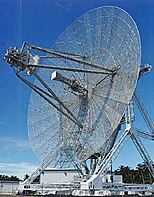
\includegraphics[width=\textwidth]{figures/Radar_antenna.jpg} 
        \caption{Radar antenna} 
        \label{fig:intro-radar} 
    \end{subfigure} 
    \begin{subfigure}[b]{0.48\textwidth} 
        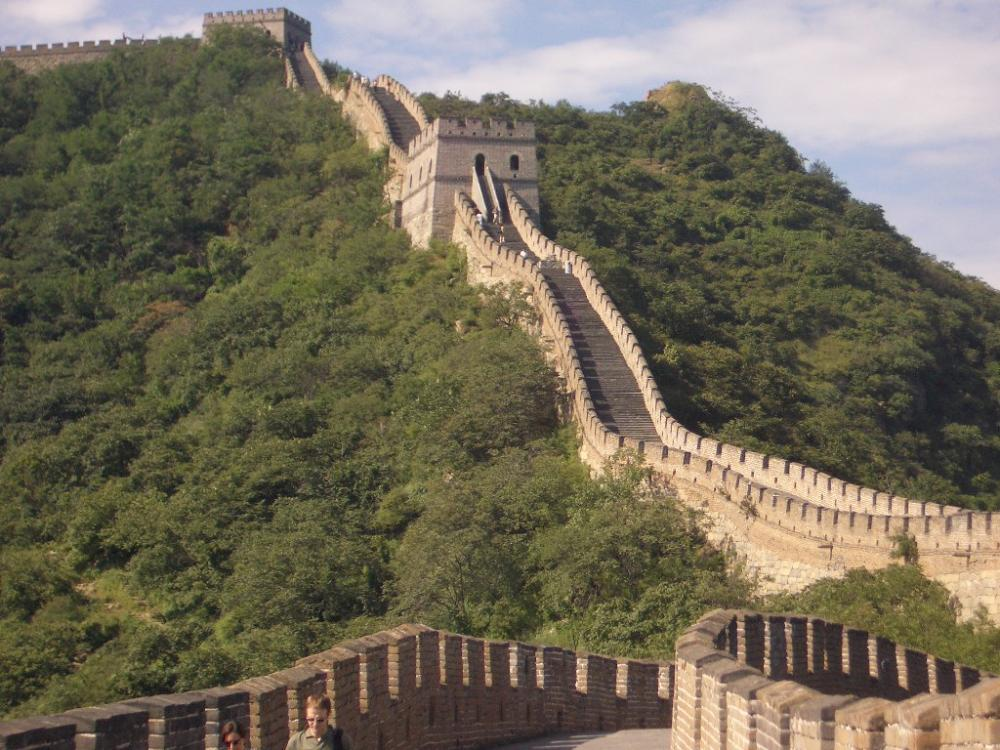
\includegraphics[width=\textwidth]{figures/great_wall.jpg} 
        \caption{Watch towers on the great wall} 
        \label{fig:intro-great_wall} 
    \end{subfigure}
    \caption{Two examples of intrusion detection system}
    \label{fig:intro-IDS}
\end{figure} 

In surveillance or tracking systems (\ref{fig:intro-laser}), 
sensors like laser beams or cameras are deployed for purposes like thief detection, 
motion capture, pose tracking and so on. 
\begin{figure}[ht] 
    \centering 
    
    % \begin{subfigure}[b]{0.55\textwidth} 
    %     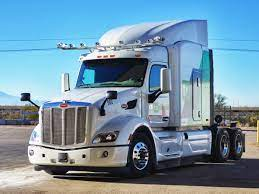
\includegraphics[width=\textwidth]{figures/truck_cam.jpeg} 
    %     \caption{Autonomous truck camera system} 
    %     \label{fig:intro_truckcam} 
    % \end{subfigure} 
    \begin{subfigure}[b]{0.41\textwidth} 
        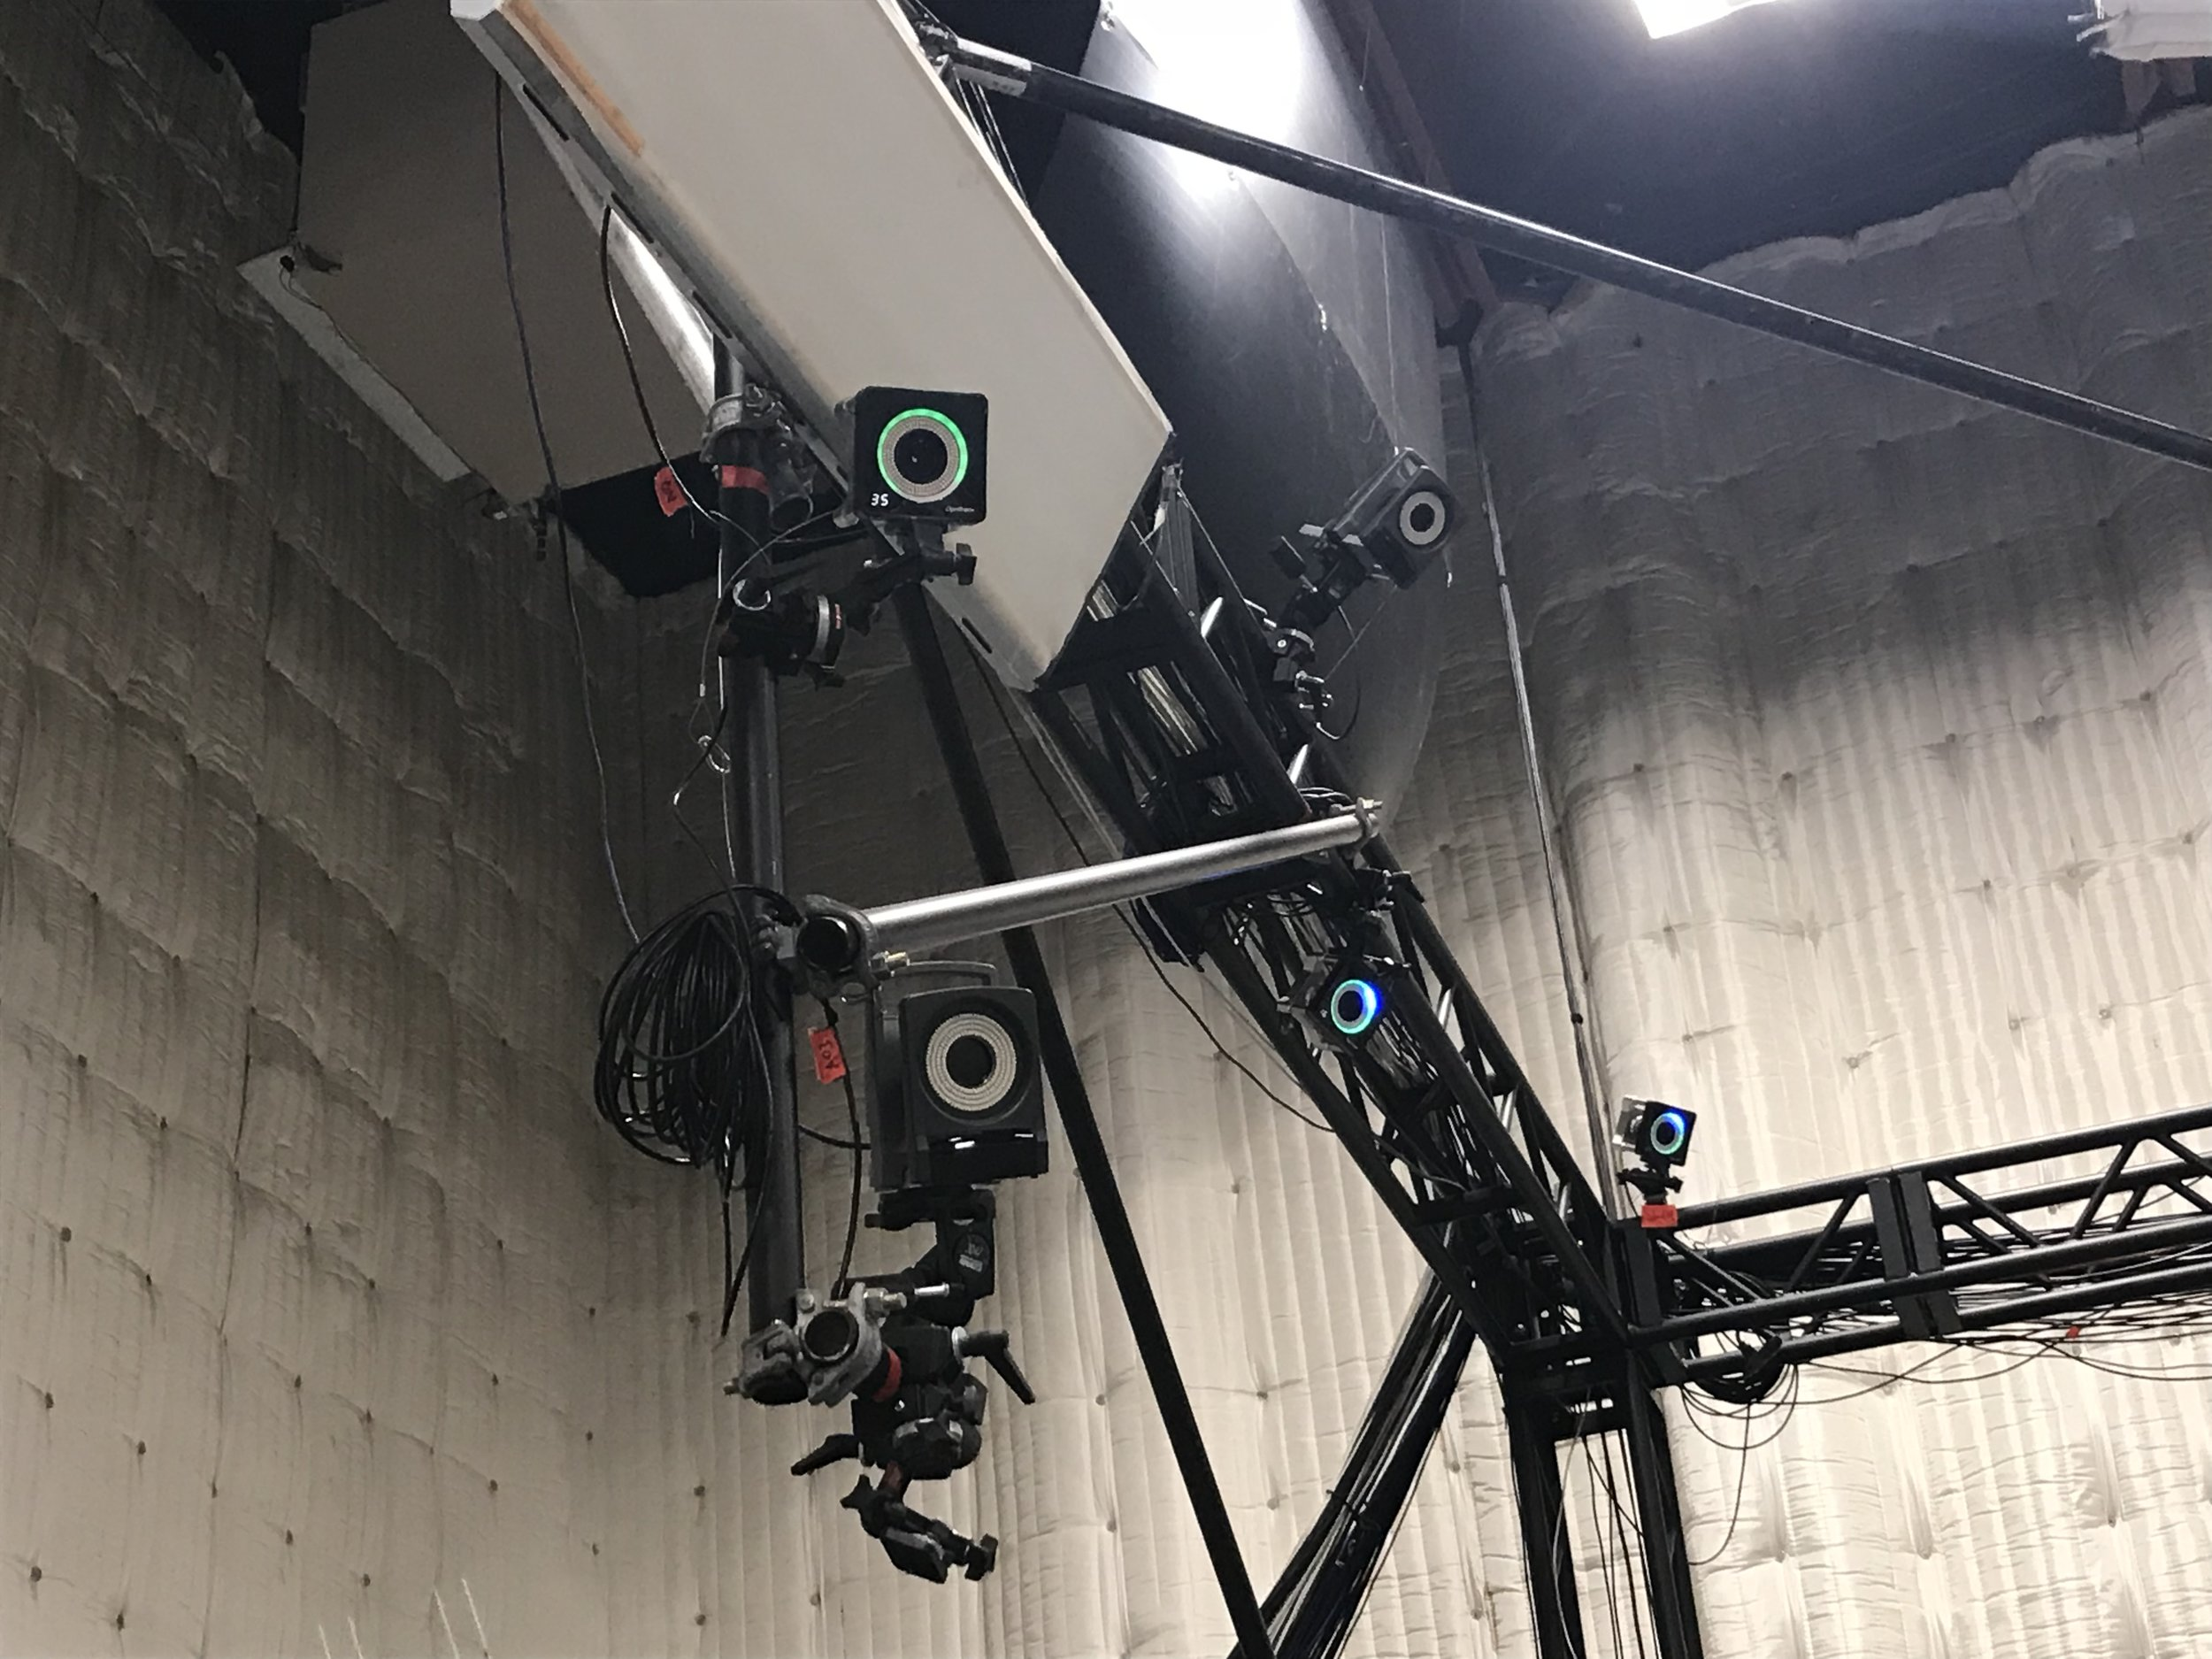
\includegraphics[width=\textwidth]{figures/optitrack.jpg} 
        \caption{Optical tracking system} 
        \label{fig:intro-optitrack} 
    \end{subfigure} 
    \hfill
    \begin{subfigure} [b]{0.46\textwidth} 
        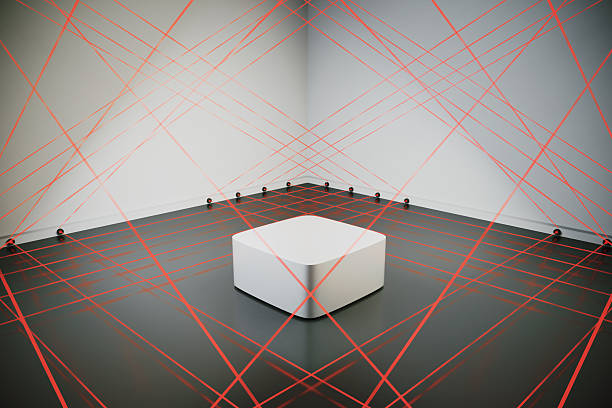
\includegraphics[width=\textwidth]{figures/laser.jpg} 
        \caption{Laser system} 
        \label{fig:intro-laser} 
    \end{subfigure} 
    \caption{Indoor tracking and surveillance systems}
    \label{fig:intro-indoor}
\end{figure}

The deployment of sensors is not limited only to deploying sensors static to the ground.
A notable example is the advent of self-driving cars.
On top of those autonomous vehicles, sensor systems are indispensable for obstacle avoidance and interactions between vehicles.
Tesla (~\ref{fig:intro-tesla}) uses 12 ultrasonic sensors 
near the front and rear bumper 
and later changed into a vision system with only cameras 
\footnote{\url{https://www.tesla.com/en_eu/support/transitioning-tesla-vision}}. 
And TuSimple, an autonomous truck company, employs a combination of cameras, radars and lidars 
for their perception system \footnote{\\\url{https://www.tusimple.com/blogs/tusimple-1000-meter-perception-system}}. 

\begin{figure}[ht] 
    \centering 

    \begin{subfigure}[b]{0.49\textwidth} 
        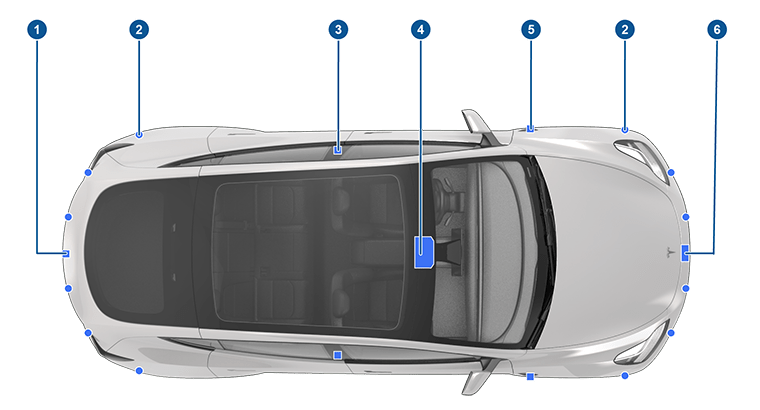
\includegraphics[width=\textwidth]{figures/tesla.png} 
        \caption{
        Tesla Model Y's sensing system
        equipped with cameras (\circled{\small{1}}, 
        \circled{\small{3}}, 
        \circled{\small{4}}, \circled{\small{5}}),
        ultrasonic sensors \circled{\small{2}}, and a radar \circled{6}.
        }
        \label{fig:intro-tesla} 
    \end{subfigure} \hfill
    \begin{subfigure}[b]{0.4\textwidth} 
        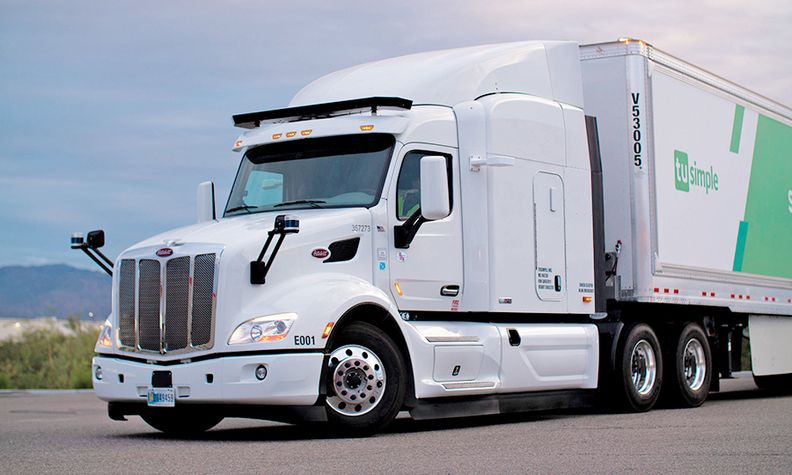
\includegraphics[width=\textwidth]{figures/tusimple.jpg} 
        \caption{TuSimple autonomous truck equipped with CMOS long-range cameras, 
        LiDARs and radars} 
        \label{fig:intro-truckcam} 
    \end{subfigure} 
    \caption{Sensor systems on autonomous vehicles}
    \label{fig:intro-autonomous-vehicles}
\end{figure} 

The placement of sensors is extremely crucial for many reasons.
First, a typical high-frequency tracking camera can cost up to several thousand US dollars in 2023, 
let alone sensors with specific industrial or military purposes. If a certain sensor layout solution
can reduce the number of sensors used in, e.g., in a secure environment, on an autonomous vehicle, or on a patrolling robot,
the cost for deployment of such sensor systems can be greatly reduced.
Second, real sensors come with many characteristics as mentioned in \cite{sebastian2005prob},
range sensors can have noise, unexpected objects blocking the view, sensing failures, random measurements and so on.
Hence, the objective that a sensor system being more balanced in terms of workload is a reasonable assumption
when quality assurance and fault tolerance are the main concerns for the system. 
Lastly, a good sensor deployment in systems like surveillance camera systems means less human labor from the security personnel;
and less energy consumption.
\section{Background}
In this section, we provide sufficient background knowledge and terms used in this dissertation, 
they will be used without explanation in the following chapters. 

\subsection{NP and NP-hardness}
% In the area of optimization, which this thesis is focusing on, NP-hardness has the 
% The definitions are taken from \cite{vazirani2001approximation}
\begin{definition}[Nondeterministic Polynomial (NP)]
    A language $L\in NP$ if there is a polynomial $p$ and a polynomial time-bounded Turing machine M, 
    called the {\textit verifier}, such that for each string $x\in \{0, 1\}^*$: 
    \begin{itemize}
        \item if $x\in L$, then there is a string $y$ (the certificate) of polynomially bounded length, i.e., $|y| \leq p(|x|)$,
        such that $M(x, y)$ accepts, and 
        \item if $x\notin L$, then for any string $y$, such that $|y|\leq p(|x|)$, $M(x,y)$ rejects.
    \end{itemize}
\end{definition}

A colloquial way in \cite{vazirani2001approximation} to describe an NP is the class of problems that have ``short and quickly verifiable'' 
Yes certificates.
% NP-complete problems refers to the class of problems such that every problem in NP can be reduced to it.
And an NP-hard problem is a problem that every problem in NP can reduce to it.
Typically, when we call an optimization problem NP-hard, it means the decision version of it is NP-hard.
\subsection{Integer programming}
Since most natural optimization problems are NP-hard, mathematical programming tools are often 
used for solving the problem for its generality and efficiency. Essentially, they take in
some mathematical models including a set of integral variables $x_1, \dots, x_n$ and a set of constraints,
\begin{align*}
    a_{11} x_{11} + \dots + & a_{1n} x_{1n} \geq b_1,\\
    \dots & \\
    a_{m1} x_{m1} + \dots + & a_{mn} x_{mn} \geq b_m,
\end{align*}
and objective 
\[
    \min a_{11} x_{11} + \dots + a_{1n} x_{1n}.
\]
When the variables $x_1, \dots, x_n$ contain continuous variables (continuum), the model becomes a mixed integer programming problem (MILP).

% e.g., its usage in Multi-robot Path Planning Problem (MRPP) \cite{HanYu19IROS, GuoHanYu21ICRA}, sensor coverage. 
Commercial (mixed) integer programming tools include Gurobi \cite{optimization2019gurobi}, IBM CPLEX \cite{cplex2009v12}, and so on,
while open-source libraries include SCIP \cite{achterberg2009scip}, CBC \cite{forrest2005cbc}, GLPK \cite{makhorin2008glpk}, and so on. 
Modern tools, even in the open-source branch, are pretty mature and developed, and hard to optimize within the framework itself. 
While work like \cite{deits2014footstep} in bipedal robot footstep planning and \cite{guo2021spatial} in multi-robot path planning 
seek performance improvement by constructing different instance formulations.

\subsection{Approximation algorithm}
For an optimization problem $\Pi$, OPT($\Pi$), or sometimes OPT, 
denotes the optimal solution of the problem instance. An $(1+\alpha)$-OPT or a $(1+\alpha)$-optimal solution refers
to a solution with an objective value of $(1+\alpha)$OPT for a minimization objective. For the maximization objective,
the corresponding term is $(1-\alpha)$OPT.

Now we give the definition of PTAS and FPTAS.
\begin{definition}[Polynomial Time Approximation Scheme (PTAS)]
    Given any $\varepsilon>0$, if an algorithm $\mathcal A$ runs in polynomial time to the input length. 
    Then if $\mathcal A$ can provide a $(1+\varepsilon)$-OPT solution, the algorithm is called PTAS.
\end{definition}

\begin{definition}[Fully Polynomial Time Approximation Scheme (FPTAS)]
    Given any $\varepsilon>0$, if an algorithm $\mathcal A$ runs in polynomial time to the input length and $1/\varepsilon$. 
    Then if $\mathcal A$ gives a $(1+\varepsilon)$-OPT solution, the algorithm is called FPTAS.
\end{definition}
\section{Problems Studied in the Dissertation}
In this section, we provide an overview of the problems studied in the later chapters, 
where each chapter is independent and self-contained. 

\begin{figure}[h]
    \centering
    \begin{subfigure}[b]{0.4\textwidth}
        \centering
        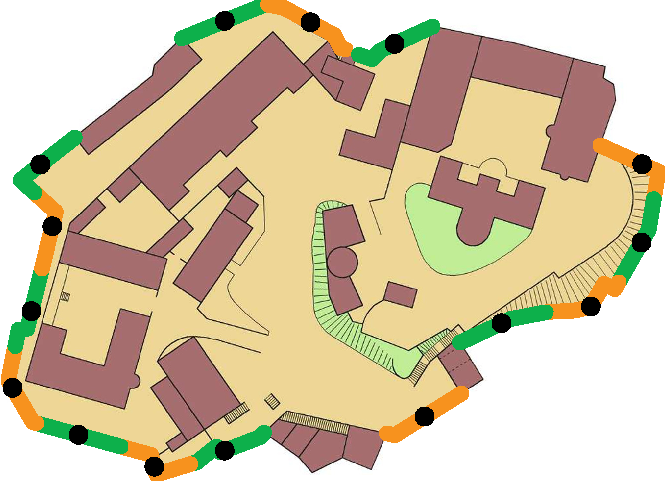
\includegraphics[width = \textwidth]{chapters/opg/figures/castle_15-eps-converted-to.pdf}
        \caption{Optimal perimeter guarding with homogeneous sensors}
        \label{fig:intro-opg-ho}
    \end{subfigure}
    \begin{subfigure}[b]{0.4\textwidth}
        \centering
        \reflectbox{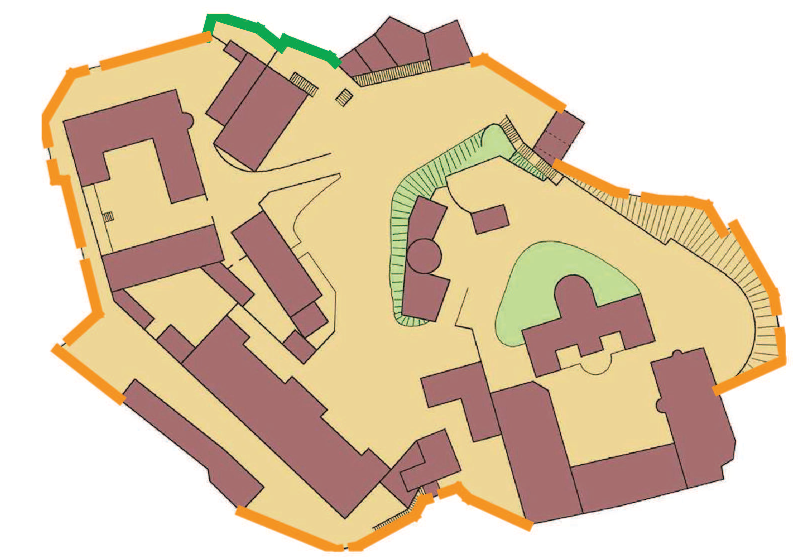
\includegraphics[width = \textwidth, angle=180]{chapters/opg-ext/figures/opgmc-castle-thin-eps-converted-to.pdf}}
        \caption{Optimal perimeter guarding with heterogeneous sensors}
        \label{fig:intro-opg-he}
    \end{subfigure}
    \caption{Optimal perimeter guarding}
    \label{fig:intro-opg}
\end{figure}


The first set of problems we studied relate to optimally assigning a larger number of sensing
robots (or other types of autonomous agents) to guard the perimeters of closed 2D regions,
where the perimeter of each region to be guarded may contain multiple disjoint polygonal chains.
Each robot is responsible for guarding a subset of the perimeter and any perimeter must be guarded
by at some robot.
The sensing range of each robot is assumed to be a continuous line on top of the perimeter of some regions. 
Specifically, two problems will be introduced, perimeter guarding with homogeneous sensors (~\ref{fig:intro-opg-ho}),
and with heterogeneous sensors (~\ref{fig:intro-opg-he}). 
The homogeneous case can be solved using only classical algorithms. 
While the heterogeneous case is NP-hard, but can still be solved with dynamic programming under a reasonable
amount of time. 


\begin{figure}[h]
    \centering
    \begin{subfigure}[b]{0.4\textwidth}
        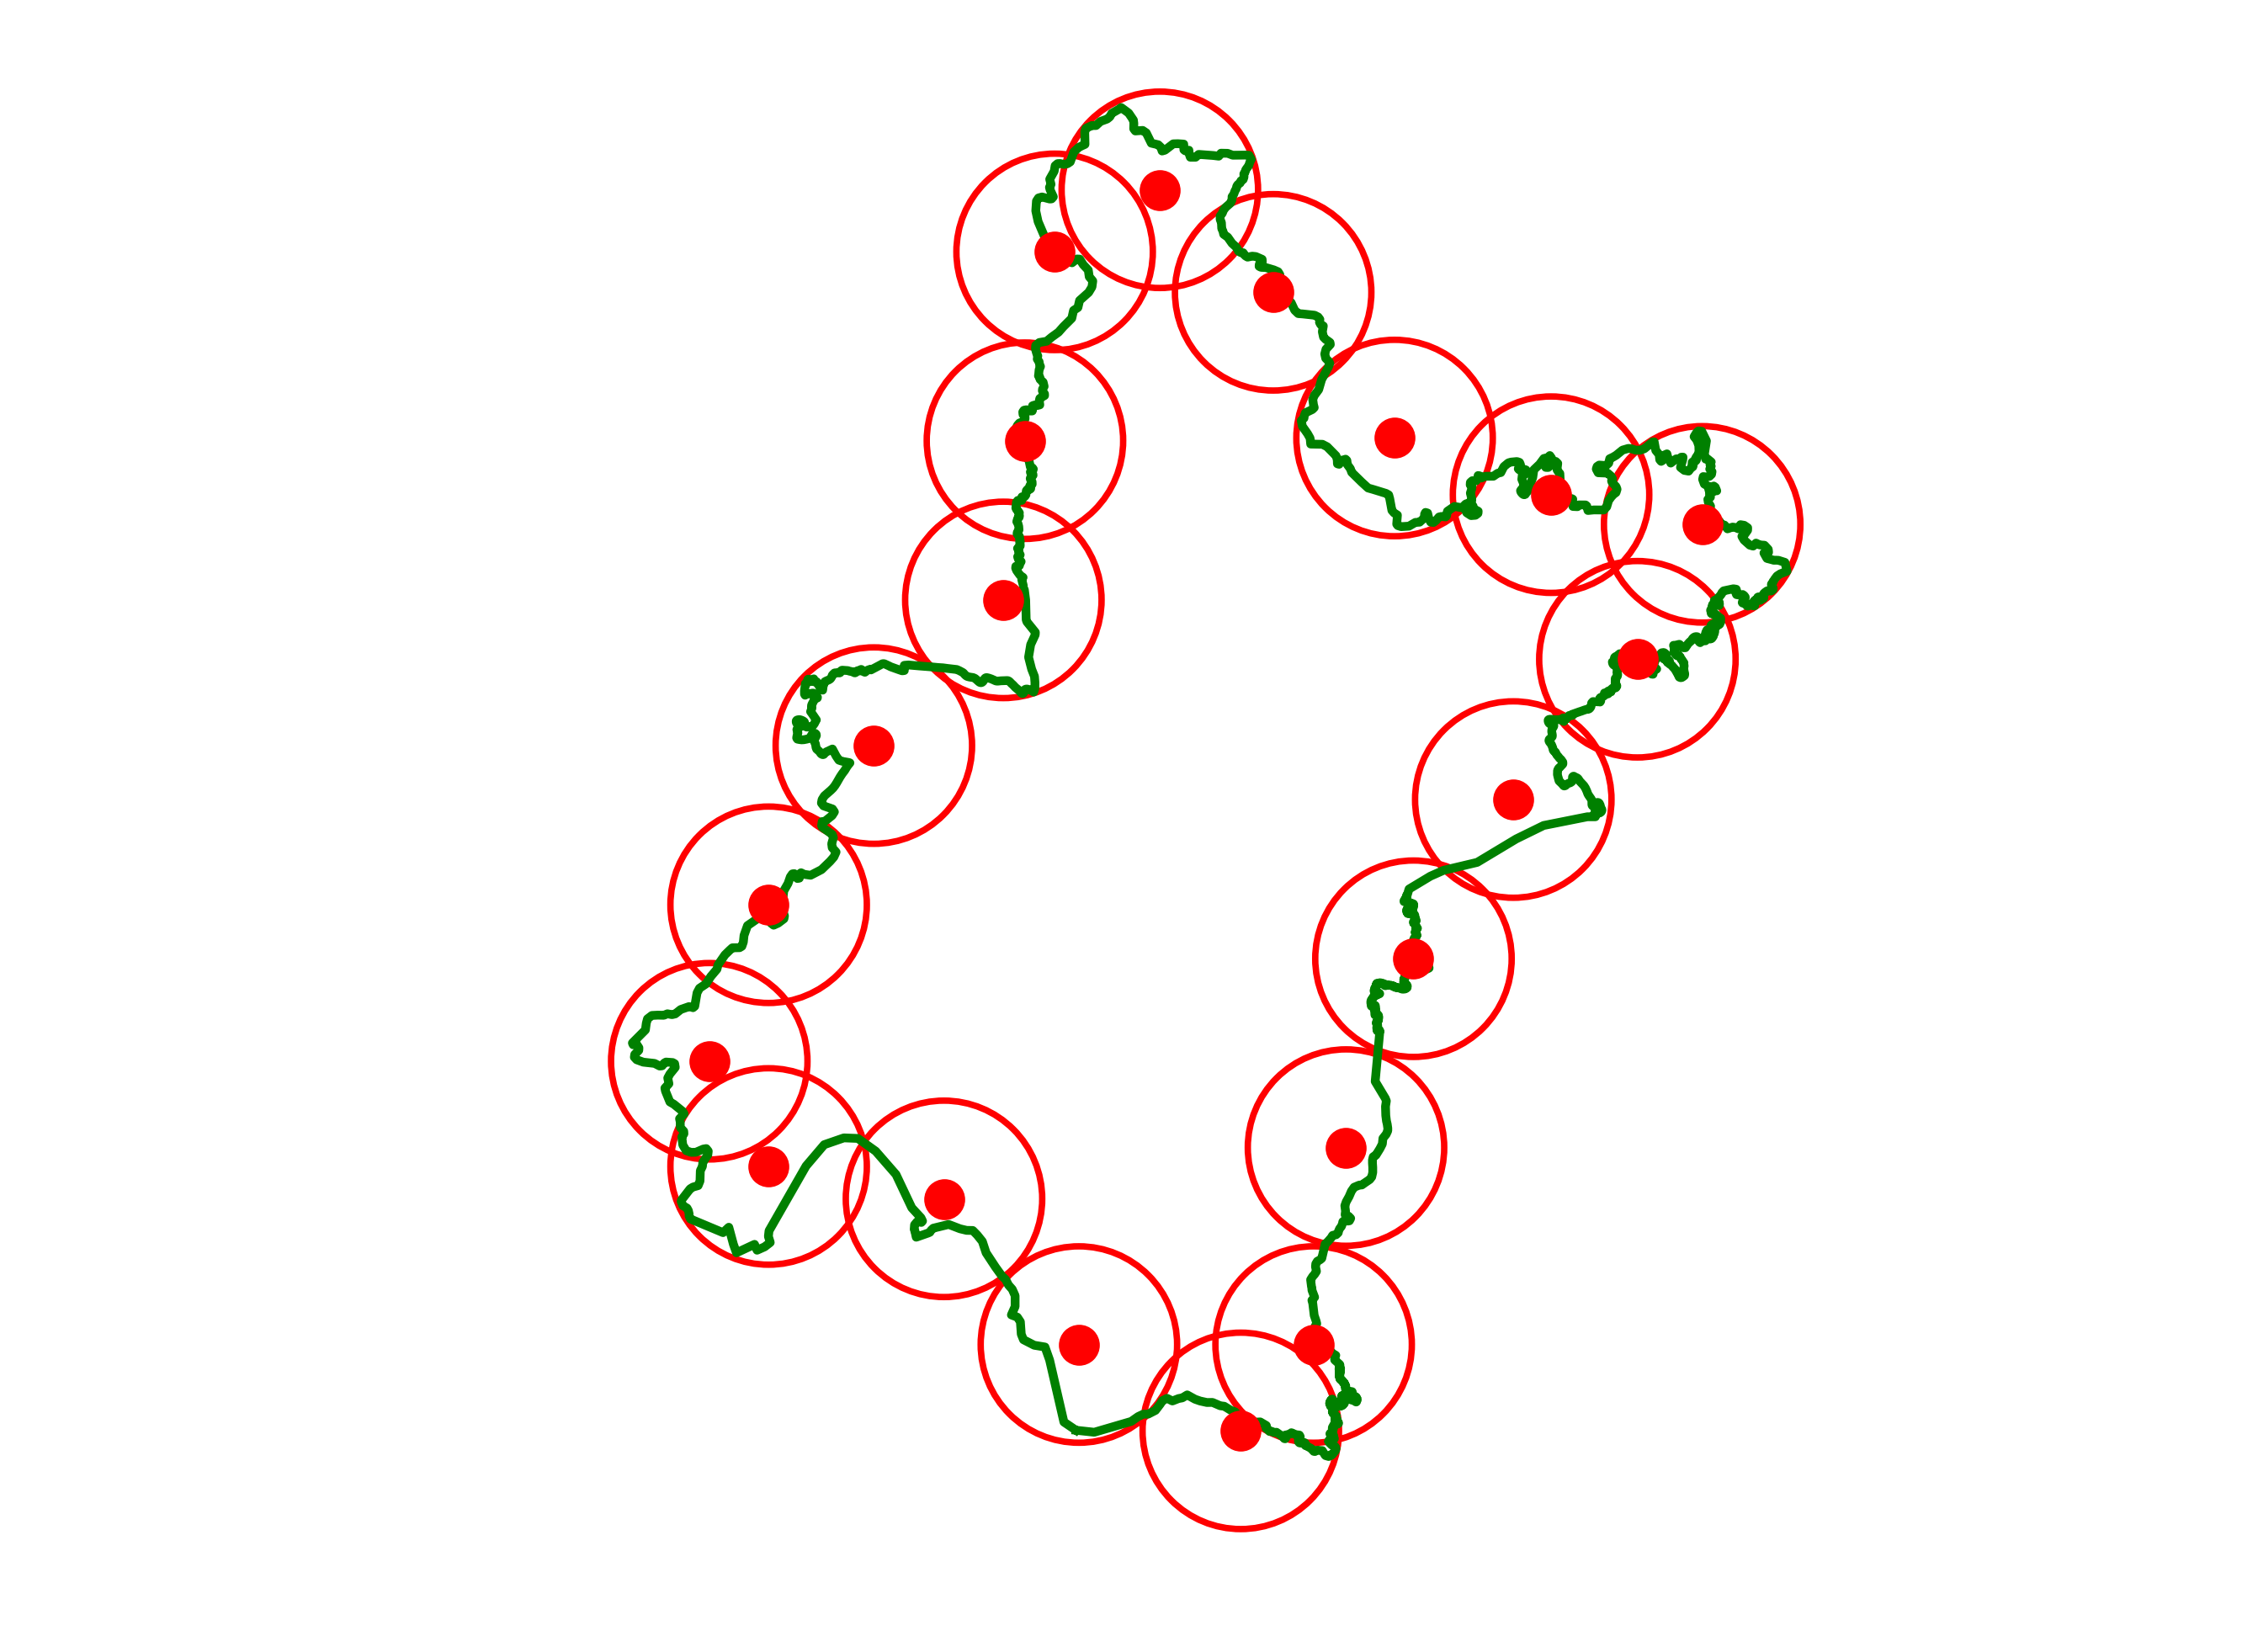
\includegraphics[width = 1.2\textwidth]{chapters/osg/figures/wuhan_ilp.png}
        \caption{Optimal perimeter guarding with 2D range sensors}
        \label{fig:intro-opg2d}
    \end{subfigure}
    \begin{subfigure}[b]{0.4\textwidth}
        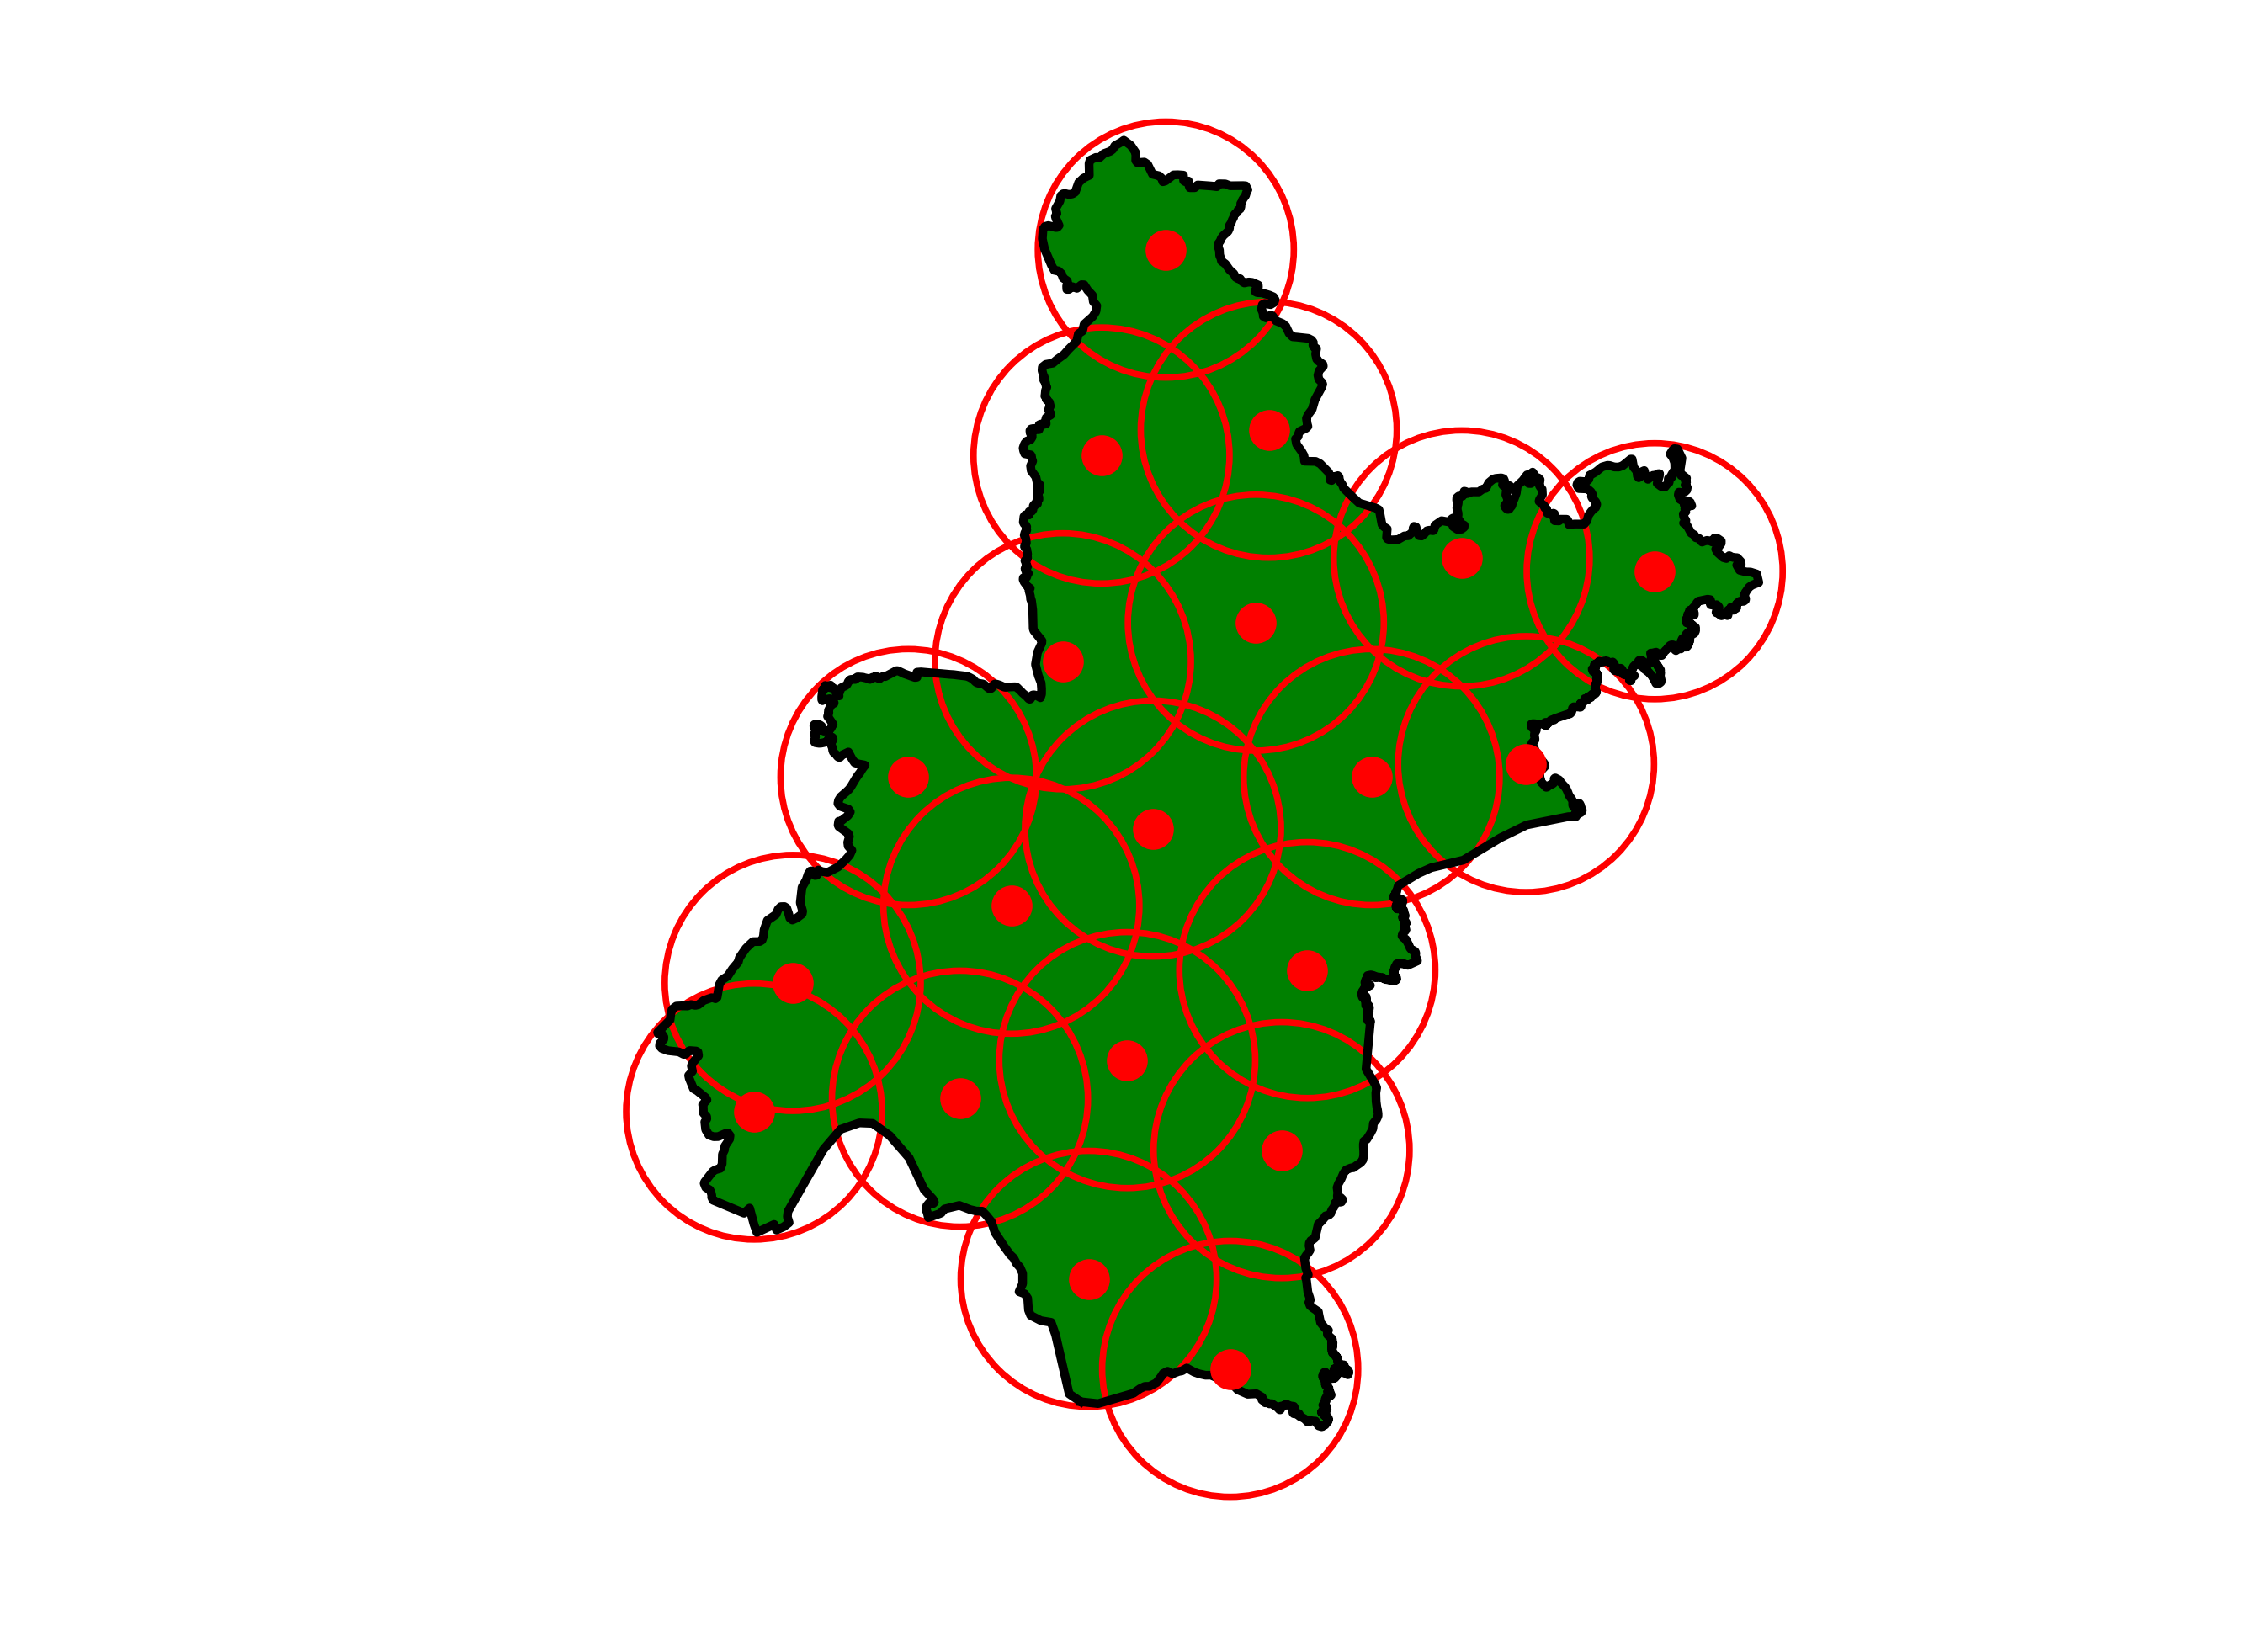
\includegraphics[width = 1.2\textwidth]{chapters/osg/figures/wuhan_region_ilp.png}
        \caption{Optimal region guarding with 2D range sensors}
        \label{fig:intro-org2d}
    \end{subfigure}
    \qquad
    \qquad
    \caption{Optimal set guarding with 20 sensors to cover the perimeter and interior of a city}
    \label{fig:intro-osg}
\end{figure}
Then, we continue with perimeter guarding but use 2D circles to represent the 
coverage range of sensors. The study extends to guarding 2D regions beyond the perimeters. 
When given a bounded $\mathbb R^2$ to be guarded, and $k$ mobile sensors with variable sensing ranges of $r_1,\dots,r_k$, 
our objective is to minimize $\max_{i=1}^{k} r_i$.
Our study shows that even for covering the boundary or interior of a simple polygon, 
the problem of finding the minimum sensing radius is NP-hard to approximate within a factor of 1.152, i.e.,
unless P=NP, there is no polynomial solution for finding a $1.152$ optimal solution. 
However, on the side of computational methods, we develop a fully polynomial time approximation algorithm for covering
a perimeter with a reasonable assumption of continuous coverage.


\begin{figure}[h]
    \centering
    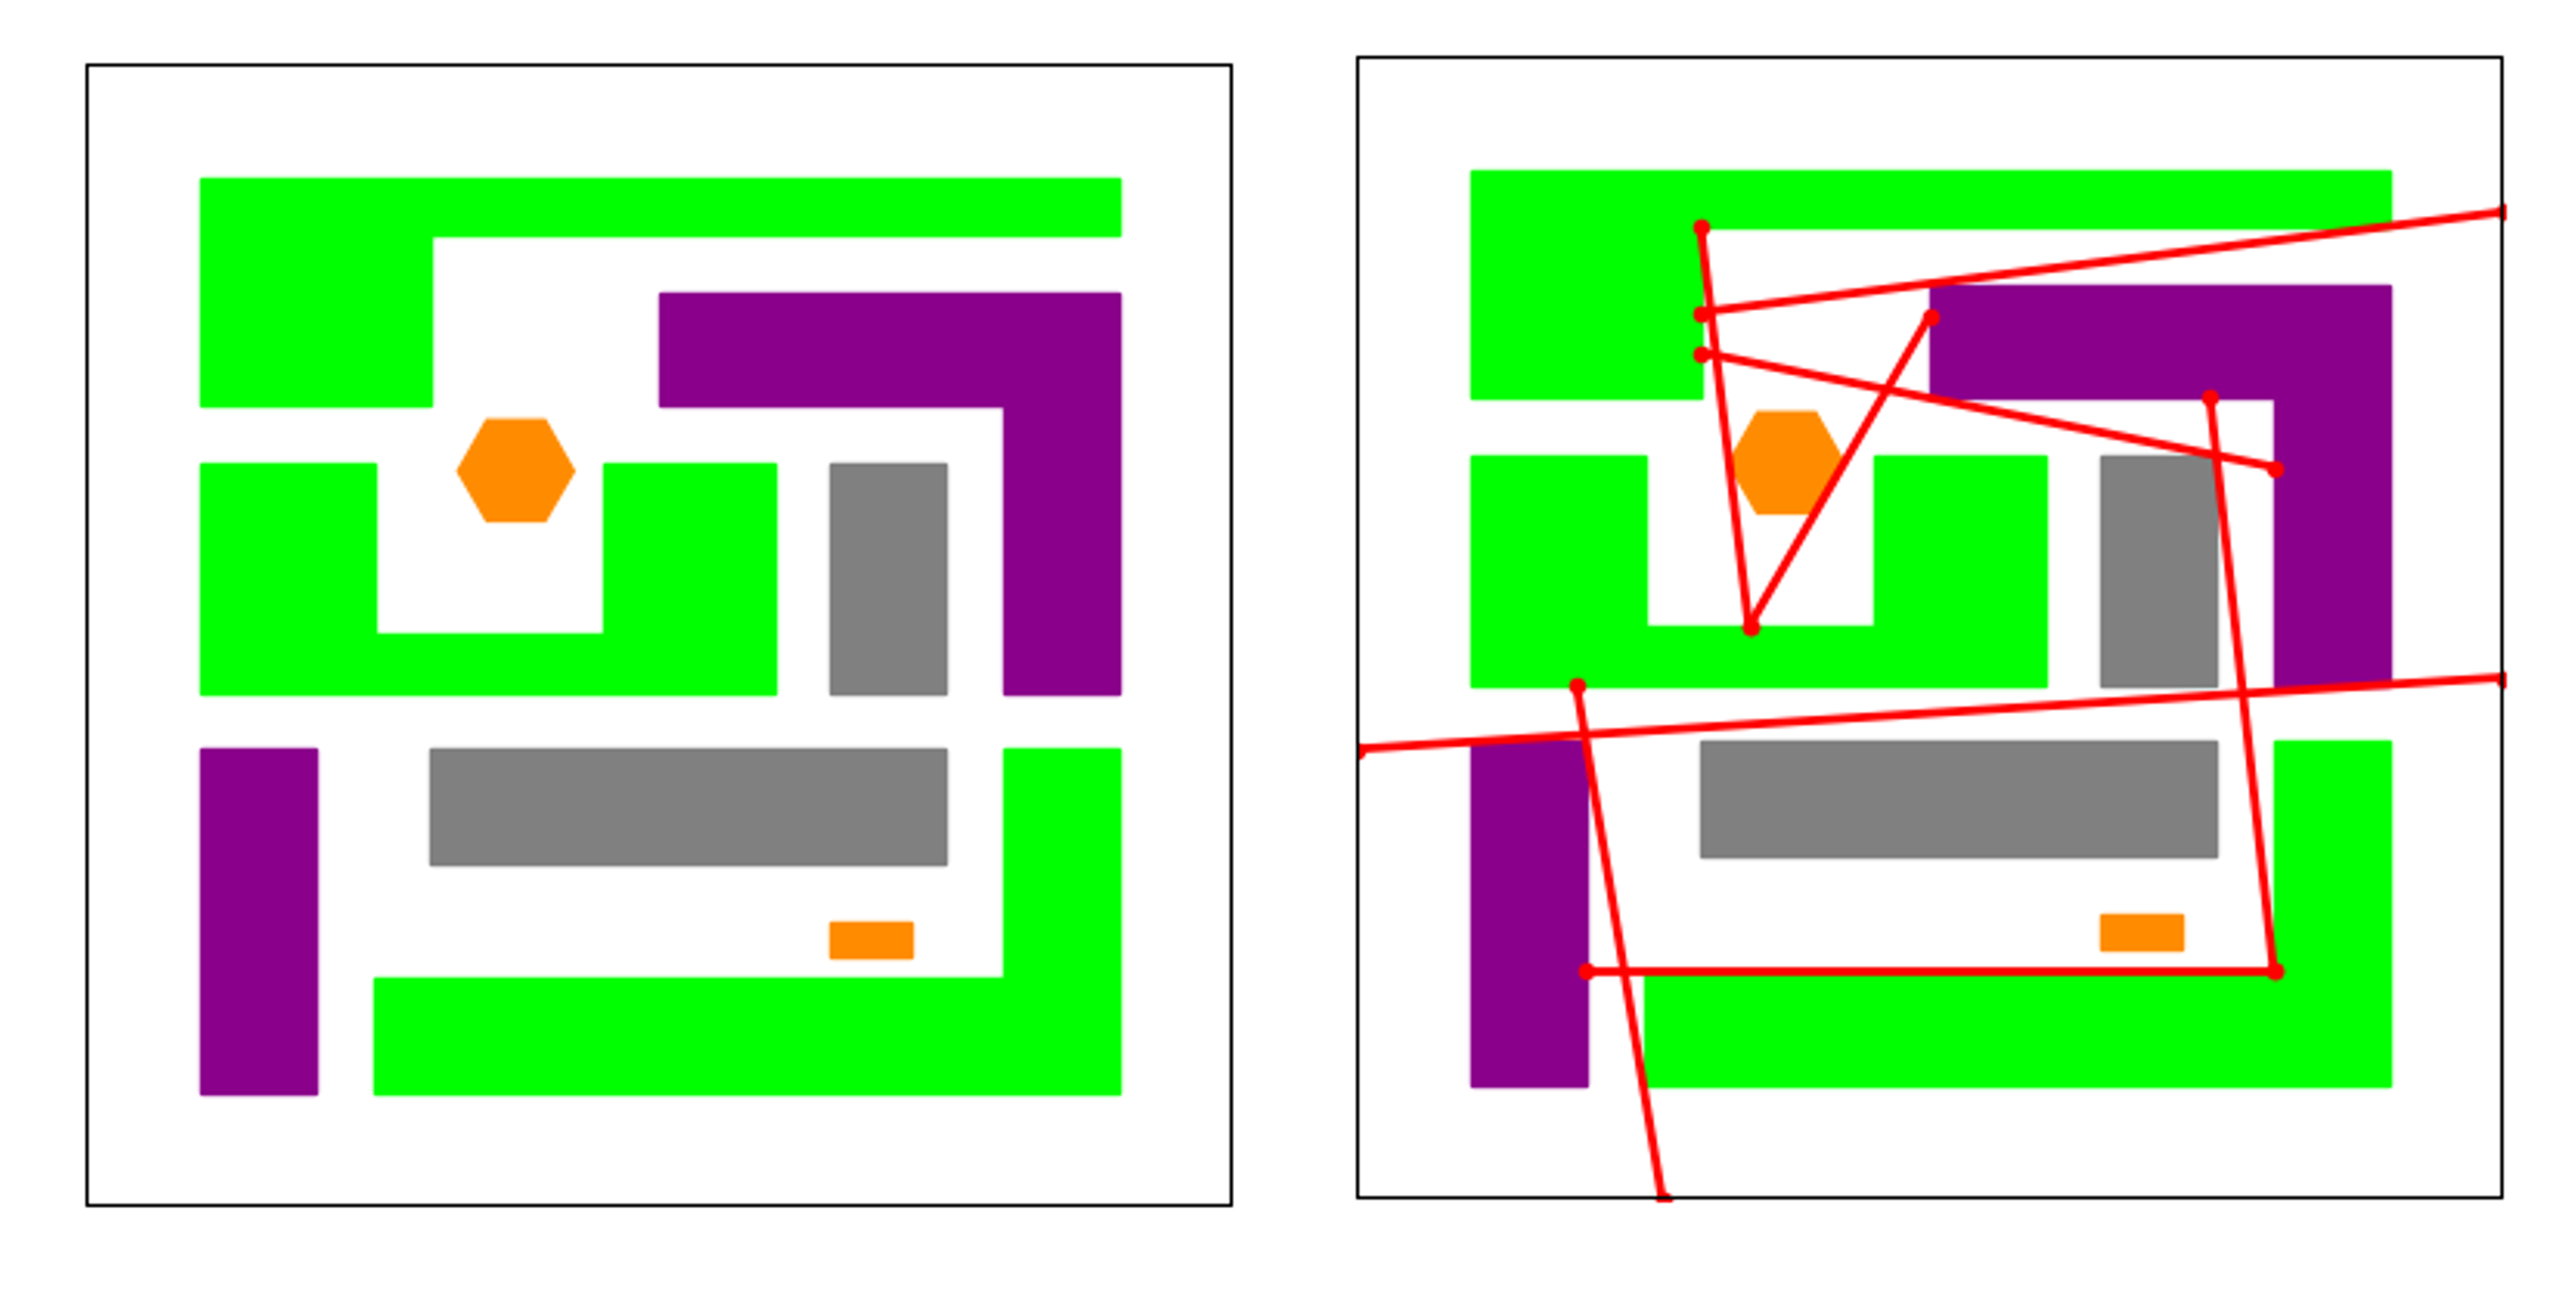
\includegraphics[width = 0.5\textwidth]{chapters/bf/fig/intro_pic.png}
    \caption[Separating three sets of building blocks with the existence of two obstacles]{Separating three sets of building blocks (orange, purple and green) with the existence of two grey obstacles.}
    \label{fig:intro-lines}
\end{figure}


After two chapters' discussion on covering perimeters or regions, which is essentially separating 
some critical polygonal regions from the outside workspace. 
The fourth chapter digs deeper into this problem by studying the separation of more than two regions. 
To simplify the problem, a line-of-sight sensing model will be adopted, where each sensor can cover
an unobstructed line segment like a laser beam. Also, the regions are assumed to be polygonal.
The objective in this case is to minimize the number of sensors used to separate these polygonal sets 
at the existence of obstacles (see ~\ref{fig:intro-lines}).
% The main objective here is to minimize the number of sensor used.
The problem is NP-hard even for the problem of separating two sets of regions with the minimum number of lines. 
Still, integer programming can provide a near-optimal solution for around 20 objects in a reasonable amount of time. 

\begin{figure}[h]
    \centering
    \vspace{-.8in}
    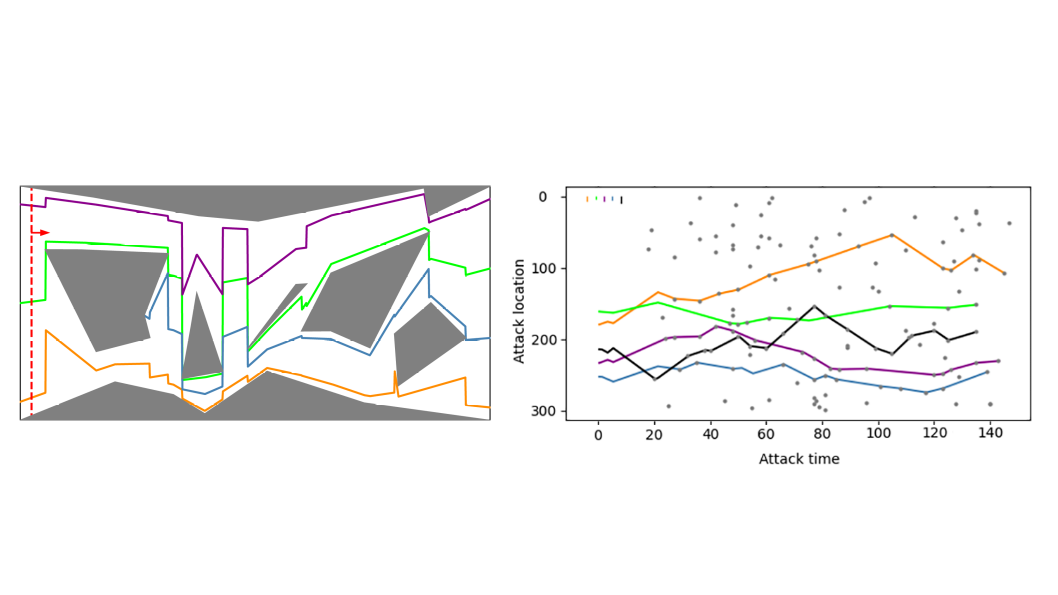
\includegraphics[width=.8\textwidth]{figures/dynamic-intro.png}
    \vspace{-.5in}
    % {
    %     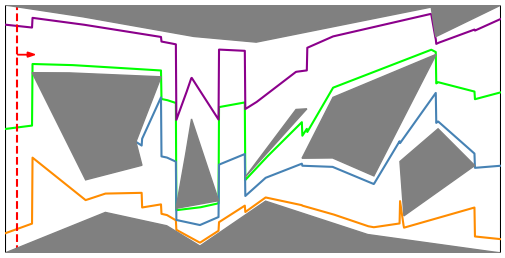
\includegraphics[width = 0.35\textwidth]{chapters/sc/fig/instance_2.png}
    % }
    % 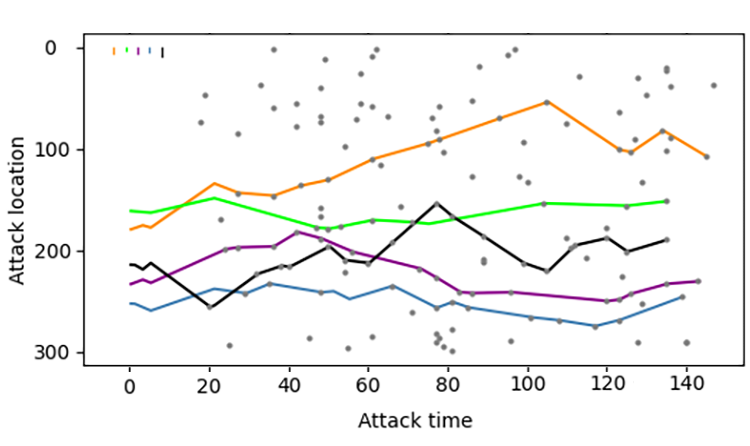
\includegraphics[width = 0.35\textwidth]{chapters/bd/fig/inf_horizon_example-v.png}
    \caption[Illustration of sweeping and boundary defense]{[left] the coordinated sweeping problem, [right] the perimeter defense problem.}
    \label{fig:intro-bd-sc}
\end{figure}

The fifth chapter deals with the dynamic setting for mobile sensing robots, 
and two different but related problems are studied. 
The first problem is the boundary defense problem in the context of heterogeneous defenders first studied in \cite{adler2022role}.
It can be seen as an extension of the perimeter defense problem \cite{shishika2020review}. 
In this problem, there are $k$ sensing robots moving on top of a perimeter with different speeds $v_1,\dots,v_k$.
A sequence of attacks $\langle loc_i, t_i \rangle_{i=1}^{n}$ are given at different time stamps and at different locations.
The objective is to intercept as many attacks as possible.
The second problem is the coordinated sweeping problem where a group of robots coordinate to sweep a region 
with obstacles. Each robot possesses a given sensing capability, and the sweeping trajectory is 
given beforehand. The objective of it is to minimize the number of robots used such that the sweeping plan 
can be executed and every point in the workspace is sensed with a certain required quality. 

\begin{figure}[ht]
    \centering
    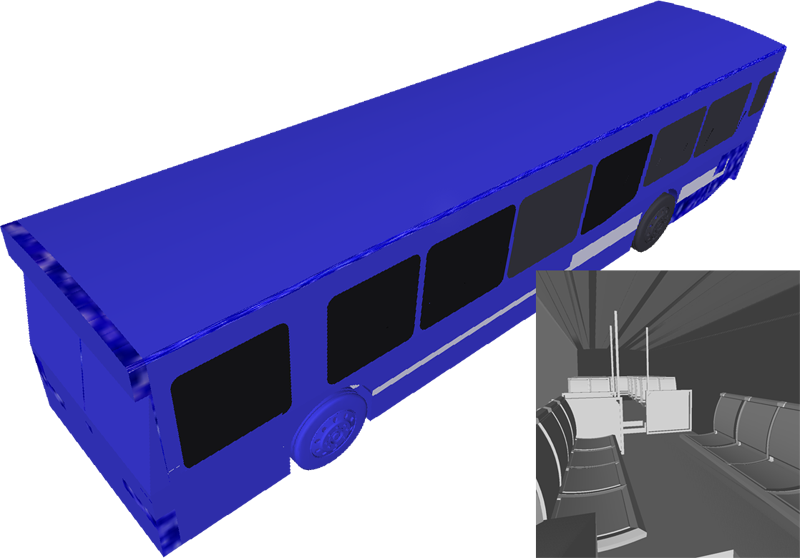
\includegraphics[width = 0.45\textwidth]{chapters/surf/fig/bus.png}
    \hfill
    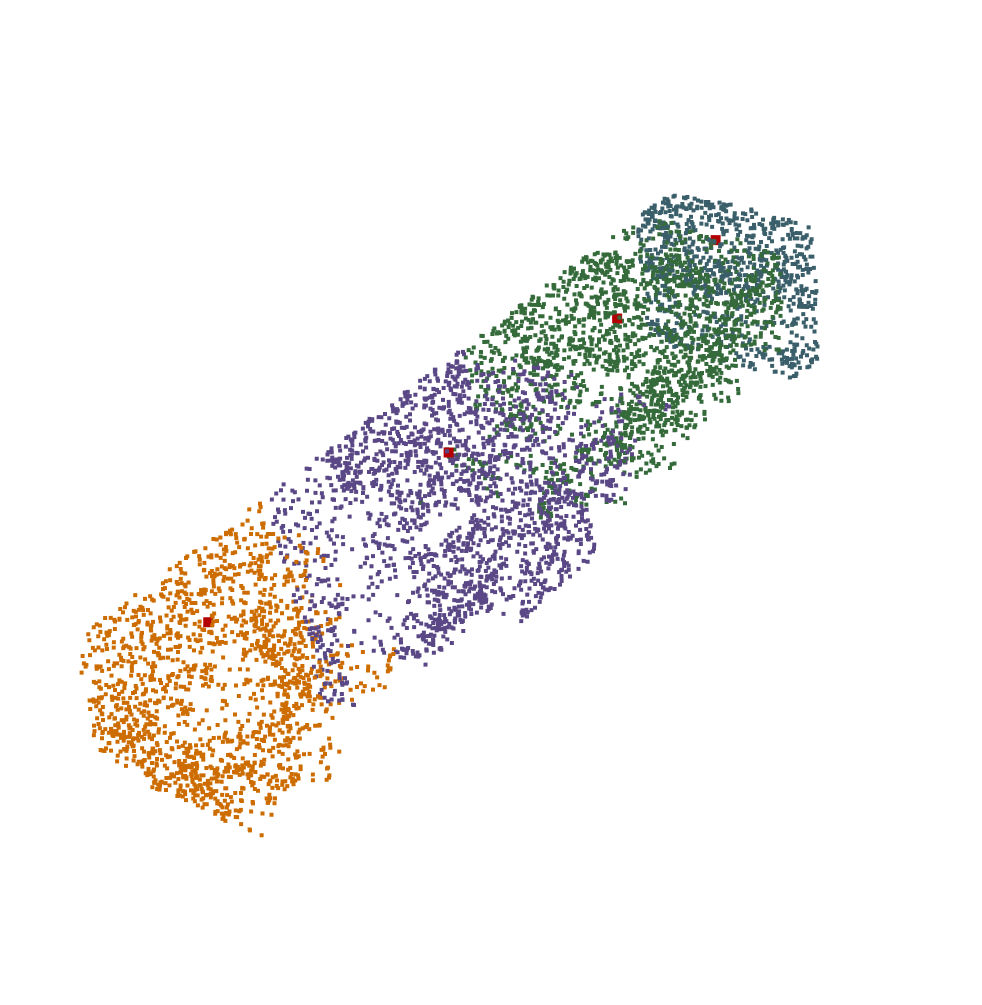
\includegraphics[width = 0.4\textwidth]{chapters/surf/fig/bus_result_3.png}
    \caption{UV sanitization lights placement to cover the interior of a bus}
    \label{fig:intro-surf}
\end{figure}

The sixth chapter discusses a real-world application in the placement of UV (ultraviolet) lights 
to cover the surface of an environment for sanitization purposes. The problem can be seen as an extension
of the art-gallery problem \cite{o1987art}, and thus computationally intractable.
Still, a combined integer programming and classical local search approach can be used to
solve the problem effectively. The method is evaluated on three real scenarios: 
the interior of a bus, a subway or an ICU room. 


\section{Literature review} 

% On the other hand, 

\subsection{Coverage-related problems in computational geometry}

As multi-robot coverage problems, this thesis is intimately connected to Art 
Gallery problems \cite{o1987art,shermer1992recent}, with origins traceable 
to half a century ago \cite{klee1969every}. Art Gallery problems assume 
a visibility-based \cite{lozano1979algorithm} sensing model; in a typical 
setup \cite{o1987art}, the {\em interior} of a polygon must be visible to at 
least one of the guards, which may be placed on the boundaries, corners, 
or the interior of the polygon. Finding the optimal number of guards are 
often NP-hard \cite{lee1986computational}. Alternatively, a disc-based sensing 
model may be used, which leads to the classical {\em packing} problem 
\cite{thue1910dichteste,hales2005proof}, where no overlap is allowed between 
the sensors' coverage area, the {\em coverage} problem 
\cite{drezner1995facility,cortes2004coverage,pavone2009equitable,martinez2010distributed,pierson2017adapting}, 
where all 
workspace must be covered with overlaps allowed, or the {\em tiling} problem 
\cite{kershner1968paving}, where the goal is to have the union of sensing
ranges span the entire workspace without overlap. For a more complete 
account on Art Gallery, packing, and covering, see Chapters 2, 3, and 33 of
\cite{toth2017handbook}. Despite the existence of a large body of literature 
performing extensive studies on these intriguing computational geometry 
problems, these types of research mostly address domains that are 2D and 
higher



% Recently, the problems of globally optimally covering perimeters using 
% one-dimensional sensors have been studied in much detail 
% \cite{fenghangaoyu2019efficient,fengyu2020RAL}. It is shown that when the sensors 
% are homogeneous, the optimal deployment of sensors can be computed 
% very efficiently, even for highly complex perimeters \cite{fenghangaoyu2019efficient}.
% On the other hand, the problem becomes immediately intractable, sometimes
% strongly NP-hard, when sensors are heterogeneous \cite{fengyu2020RAL}. 
% Our research is distinct from \cite{fenghangaoyu2019efficient,fengyu2020RAL} in that 
% we employ a (two-dimensional) range sensing model and work on the coverage 
% of both perimeters and regions, which has much broader applicability. 

As pointed out in \cite{cortes2004coverage,schwager2009decentralized}, 
distributed sensor coverage has roots in the study 
of the facility location optimization problem 
\cite{weber1929theory,drezner1995facility}, which examines the selection 
of facility (e.g., warehouses) locations that minimize the cost of delivery 
of supplies to spatially distributed customers. In theoretical computer 
science and operations research, these are known as the $k$-center, 
$k$-means, and $k$-median clustering problems \cite{har2011geometric}, 
the differences among which are induced by the cost structure. Our 
investigations benefit from the vast literature on 
the study of $k$-center clustering and related problems, e.g., 
\cite{feder1988optimal,hochbaum1985best,gonzalez1985clustering,daskin2000new,shamos1975closest}.
%
These clustering problems are in turn related to packing 
\cite{hales2005proof}, tiling \cite{thue1910dichteste}, and the 
well-studied art gallery problems \cite{o1987art,shermer1992recent}.

% \subsection{Mobile sensing robot coverage control} 
\subsection{Multi-robot coordination} 
Our work draws inspiration from a long line of multi-robot coverage planning and 
control research, e.g., \cite{cortes2004coverage,martinez2007motion,
schwager2009optimal,pavone2009equitable,schwager2009decentralized,
pierson2017adapting}. 
%
In an influential body of work on coverage control \cite{cortes2004coverage,
martinez2007motion}, a gradient-based iterative method is shown to drive 
one or multiple mobile sensors to a locally optimal configuration with 
convergence guarantees. 
%
Whereas \cite{cortes2004coverage,martinez2007motion} assume that the 
distribution of sensory information is available {\em a priori}, it is 
shown that such information can be effectively learned 
\cite{schwager2009decentralized}. 
%
Subsequently, the control method is further extended to allow the 
coverage of non-convex and disjoint 2D domains \cite{schwager2009optimal} 
and to work for mobile robots with varying sensing or actuation capabilities
\cite{pierson2017adapting}. 
%
In contrast to these control-based approaches, which produce iterative 
locally optimal solutions, our work emphasizes the direct computation of 
globally optimal deployment solutions and supports arbitrarily shaped
bounded (1D) perimeters and (2D) regions.

With an emphasis on robotic swarm deployment, within multi-robot 
systems research \cite{arai2002advances,gerkey2004formal,ren2008distributed,bullo2009distributed}, 
our study is closely related to {\em formation control}, e.g., 
\cite{ando1999distributed,jadbabaie2003coordination,olfati2004consensus,ren2005consensus,cheng2008almost,mesbahi2010graph,yu2012rendezvous},
where the goal is to achieve certain {\em distributions} through 
continuous (often, local sensing based) interactions among the 
agents or robots. Depending on the particular setting, the 
distribution in question may be spatial, e.g., rendezvous
\cite{ando1999distributed,yu2012rendezvous}, or maybe an agreement 
in agent velocity is sought \cite{jadbabaie2003coordination,ren2005consensus}. 
In these studies, the resulting formation often have some 
degree-of-freedoms left unspecified. For example, rendezvous 
results \cite{ando1999distributed,yu2012rendezvous} often come 
with exponential convergence guarantee, but the location of
rendezvous is generally unknown {\em a priori}. 

In multi-robot task and motion planning problems (e.g.,
\cite{smith2009monotonic,ayanian2010decentralized,liu2011multi,liu2013optimal,turpin2014goal,turpin2014capt,alonso2015multi,SolYu15}), 
especially ones with a {\em task allocation} element 
\cite{smith2009monotonic,liu2011multi,liu2013optimal,turpin2014goal,turpin2014capt,SolYu15},
the (permutation-invariant) target configuration is often mostly 
known. The goal here is to find a one-to-one mapping between individual 
robots and the target locations (e.g., deciding a {\em matching}) and 
then plan (possibly collision-free) trajectories for the robots to reach 
their respective assigned targets \cite{turpin2014goal,turpin2014capt,SolYu15}.  

\subsection{Search and rescue}
The study of the dynamic coverage in this dissertation draws inspiration from the study of several 
lines of related problems. 
The Graph-Clear problem, formulated in \cite{kolling2007graph}, tasks a group of robots to search and clear an environment with the operations of blocking and clearing.
A follow-up work on Line-Clear \cite{kolling2017coordinated} uses line guards
with more focus on computational geometry in that
the objective is to minimize the maximum sweep line distance. Both of these problems are
NP-hard, establishing the difficulties of finding a sweeping schedule for a planar environment.
The more general pursuit-evasion problem dates back to the research on \emph{search number}
on a discrete graph \cite{megiddo1988complexity}, 
followed by studies on pursuit and evasion in continuous environments with 
visibility-based model \cite{guibas1999visibility, suzuki1992searching, lavalle2000algorithm, stiffler2017persistent}. 

When working with known patrolling search frontiers, e.g., vertical sweep lines, 
this sweep line coverage problem is analogous to the perimeter defense problem by placing guards on a static perimeter
to defend intruders \cite{shishika2020cooperative, macharet2020adaptive, chen2021optimal}.
Previously, we have also studied a version of static range guard placement problems for securing perimeters and regions \cite{fengyu2020optimally}.
In contrast to the pursuit-evasion algorithms that deal with searching dynamic and unpredictable targets that could escape, 
coverage planning/control-related algorithms become more suitable for searching or covering predictable or stationary targets,
e.g., room sweeping, pesticide and fertilizer spraying, persistent monitoring, and so on 
\cite{cortes2004coverage, Correia2021icra, oksanen2009coverage, haksar2020spatial, wei2018coverage, deng2019constrained, 
lan2013planning, cassandras2012optimal, yu2015persistent, palacios2017optimal}. 

% The problem becomes the well-known art-gallery problem \cite{o1987art} when a static deployment of robots is sought after.
% In contrast to formation control and multi-robot motion planning research, 
% our study of \opg seeks to determine an exact, optimal distribution 
% pattern of robots (in this case, over a fairly arbitrary, bounded 1D 
% topological domain). Thus, solutions to \opg may serve as the target 
% distributions for multi-robot task and motion planning, which is a main 
% motivation behind our work. The generated distribution pattern is 
% also potentially useful in multi-robot persistent monitoring 
% \cite{soltero2014decentralized} and coverage \cite{howard2002mobile,schwager2009optimal} 
% applications, where robots are asked to carry out sensing tasks in some 
% optimal manner. 
% \subsection{Sensor network} 

% \section{Application}
